\documentclass{beamer}
\mode<presentation>
\usepackage{amsmath}
\usepackage{amssymb}
%\usepackage{advdate}
\usepackage{adjustbox}
\usepackage{subcaption}
\usepackage{enumitem}
\usepackage{multicol}
\usepackage{mathtools}
\usepackage{listings}
\usepackage{url}
\def\UrlBreaks{\do\/\do-}
\usetheme{Boadilla}
\usecolortheme{lily}
\setbeamertemplate{footline}
{
  \leavevmode%
  \hbox{%
  \begin{beamercolorbox}[wd=\paperwidth,ht=2.25ex,dp=1ex,right]{author in head/foot}%
    \insertframenumber{} / \inserttotalframenumber\hspace*{2ex} 
  \end{beamercolorbox}}%
  \vskip0pt%
}
\setbeamertemplate{navigation symbols}{}

\providecommand{\nCr}[2]{\,^{#1}C_{#2}} % nCr
\providecommand{\nPr}[2]{\,^{#1}P_{#2}} % nPr
\providecommand{\mbf}{\mathbf}
\providecommand{\pr}[1]{\ensuremath{\Pr\left(#1\right)}}
\providecommand{\qfunc}[1]{\ensuremath{Q\left(#1\right)}}
\providecommand{\sbrak}[1]{\ensuremath{{}\left[#1\right]}}
\providecommand{\lsbrak}[1]{\ensuremath{{}\left[#1\right.]}}
\providecommand{\rsbrak}[1]{\ensuremath{{}\left.[#1\right]}}
\providecommand{\brak}[1]{\ensuremath{\left(#1\right)}}
\providecommand{\lbrak}[1]{\ensuremath{\left(#1\right.)}}
\providecommand{\rbrak}[1]{\ensuremath{\left.#1\right)}}
\providecommand{\cbrak}[1]{\ensuremath{\left\{#1\right\}}}
\providecommand{\lcbrak}[1]{\ensuremath{\left{#1\right.}}}
\providecommand{\rcbrak}[1]{\ensuremath{\left.{#1\right.}}}
\theoremstyle{remark}
\newtheorem{rem}{Remark}
\newcommand{\sgn}{\mathop{\mathrm{sgn}}}
\providecommand{\abs}[1]{\left\vert#1\right\vert}
\providecommand{\res}[1]{\Res\displaylimits_{#1}} 
\providecommand{\norm}[1]{\lVert#1\rVert}
\providecommand{\mtx}[1]{\mathbf{#1}}
\providecommand{\mean}[1]{E\left[ #1 \right]}
\providecommand{\fourier}{\overset{\mathcal{F}}{ \rightleftharpoons}}
%\providecommand{\hilbert}{\overset{\mathcal{H}}{ \rightleftharpoons}}
\providecommand{\system}{\overset{\mathcal{H}}{ \longleftrightarrow}}
	%\newcommand{\solution}[2]{\textbf{Solution:}{#1}}
%\newcommand{\solution}{\noindent \textbf{Solution: }}
\providecommand{\dec}[2]{\ensuremath{\overset{#1}{\underset{#2}{\gtrless}}}}
\newcommand{\myvec}[1]{\ensuremath{\begin{pmatrix}#1\end{pmatrix}}}
\let\vec\mathbf

\lstset{
%language=C,
frame=single, 
breaklines=true,
columns=fullflexible
}

\numberwithin{equation}{section}

\title{Presentation Template}
\author{M. Rajesh Kumar Reddy\\EE24BTECH11043\\ Dept. of Electrical Engg.,\\IIT Hyderabad.}

\date{\today} 
\begin{document}

\begin{frame}
\titlepage
\end{frame}

\section*{Outline}
\begin{frame}
\tableofcontents
\end{frame}
\section{Problem}
\begin{frame}
\frametitle{Problem Statement}
	Find the point which divides the line segment joining the points $\vec{P}\brak{7,-6}$ and $\vec{Q}\brak{3,4}$ in the ratio $1:2$ internally and the quadrant in which it lies using section formula.
\end{frame}

%\subsection{Literature}
\section{Solution}
\subsection{Section Formula}
\begin{frame}
\frametitle{Section Formula}
%\framesubtitle{Literature}
%
Let the point which divides $\vec{P}$ and $\vec{Q}$ in the ratio $1:2$ be $\vec{R}$.
%
By using Section Formula
	\begin{align}
		\vec{R} = \frac{2\times\vec{P}+1\times\vec{Q}}{1+2} \\
		\vec{R}\myvec{x\\y} = \frac{2}{3}\myvec{7\\-6} + \frac{1}{3}\myvec{3\\4} \\
		\vec{R}\myvec{x\\y} =\frac{1}{3}\myvec{17\\-8} \\
		\vec{R}\myvec{x\\y} =\myvec{\frac{17}{3}\\ \frac{-8}{3}} 
	\end{align}
\end{frame}
\section{Plot}
\subsection{Plot- Using Python-code}
\begin{frame}
\frametitle{Plot Points in Graph}

		\begin{figure}[H]
	\centering
				\begin{minipage}{1\textwidth}
	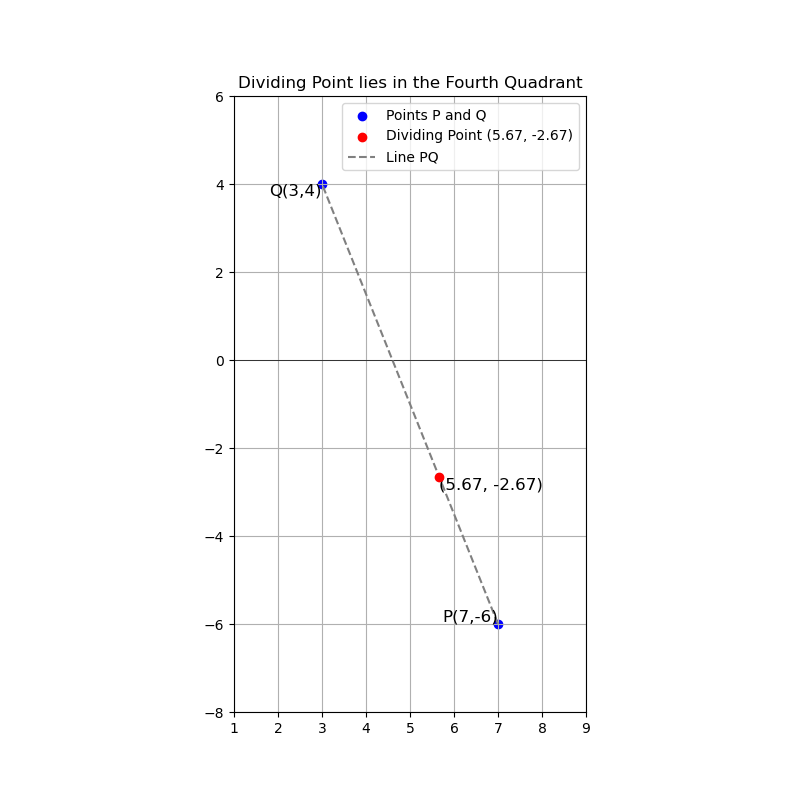
\includegraphics[width=0.7\linewidth]{figs/Plot.png}
			\end{minipage}
			\end{figure}
			
\end{frame}
\section{Codes}
\subsection{C-code}
\begin{frame}
\frametitle{C-code}
	C-code shown below is used to find the point $\vec{R}$ and the quadrant in which it lies.
             	\begin{figure}[H]
	\centering
				\begin{minipage}{0.5\textwidth}
	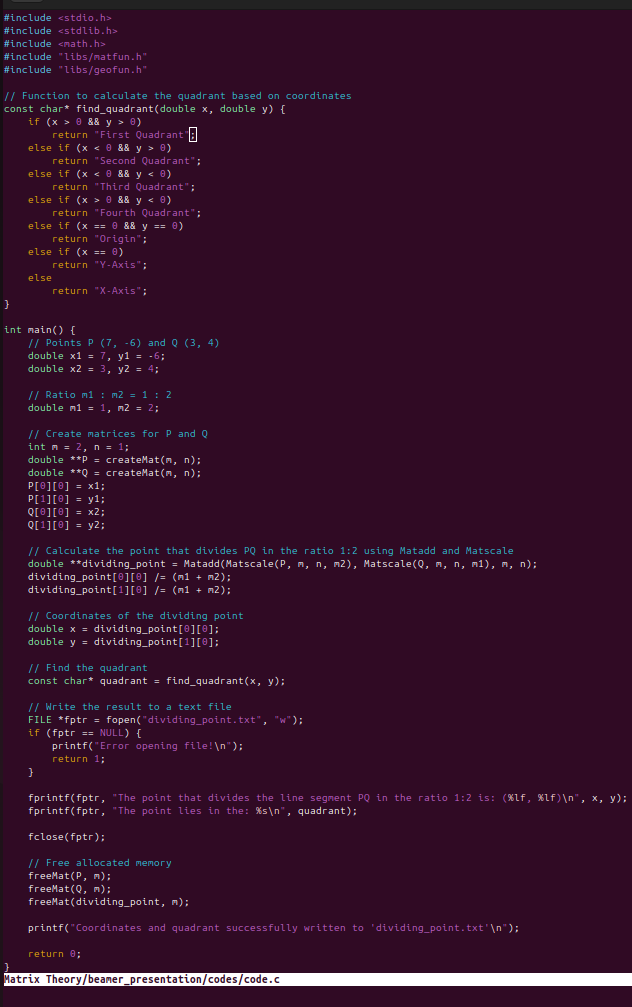
\includegraphics[width=0.7\linewidth]{figs/C-code.png}
			\end{minipage}
			\end{figure} 

\end{frame}
\subsection{Python code}
\begin{frame}[fragile]
\frametitle{Python code}
Python code reads the point and plots in graph
                 	\begin{figure}[H]
	\centering
				\begin{minipage}{0.5\textwidth}
	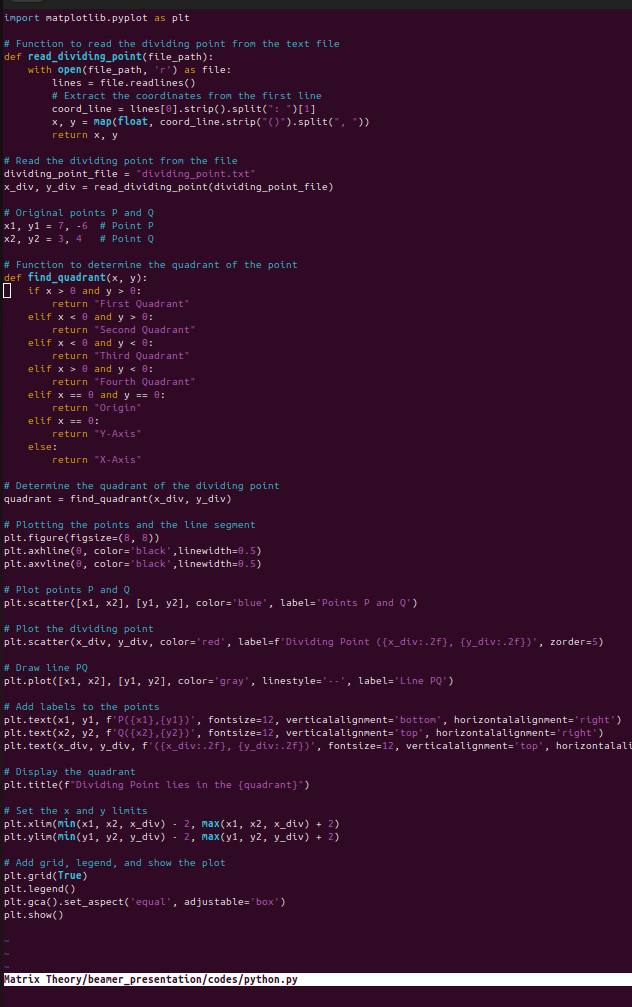
\includegraphics[width=0.7\linewidth]{figs/Py-code.png}
			\end{minipage}
			\end{figure}


\end{frame}
\end{document}

